\section{Preliminaries}
In this section, we first introduce the preliminaries for tweets in both scenarios. Our system will continuously monitor the Twitter's live tweet sample stream using the official API. As soon as the system obtains the json data of tweets, the system will preprocess the tweet text and filter tweets without any keywords in each user's profile.

\subsection{Pre-processing}
The preprocessing we adopt on tweet stream is described as follows:
\begin{itemize}
\item \textbf{Non-English Filtering:} Tweets written in a language other than English would be judged as not relevant based on guidelines of Real-Time Summarization Track. Thus, we use the twitter's language detector to abandone the non-English tweets.
\item \textbf{Non-ASCII Words:} Removing all NON-ASCII characters from the tweets will also helps remove non-English tweets.
\item \textbf{Redundant Retweet Elimination:} All additional commentary in the tweets containing 'RT @' will be ignored. As the guidline mentioned, all retweets should be normalized to the underlying tweets.
\item \textbf{Porter Stemming and Stopword Filtering:} We remove all stopwords and stem the tweet text using the Natural Language Toolkit.
\end{itemize}

\subsection{Filtering}
In order to boost the speed of identifying possible relevant tweets for each user's interest profile $q$, we simply filter tweets that do not contain any keywords for each profile $q$, and the rest tweets are chosen as candidate tweet collection $\Gamma$ for $q$.

\begin{figure}[htbp]
\centering
{
	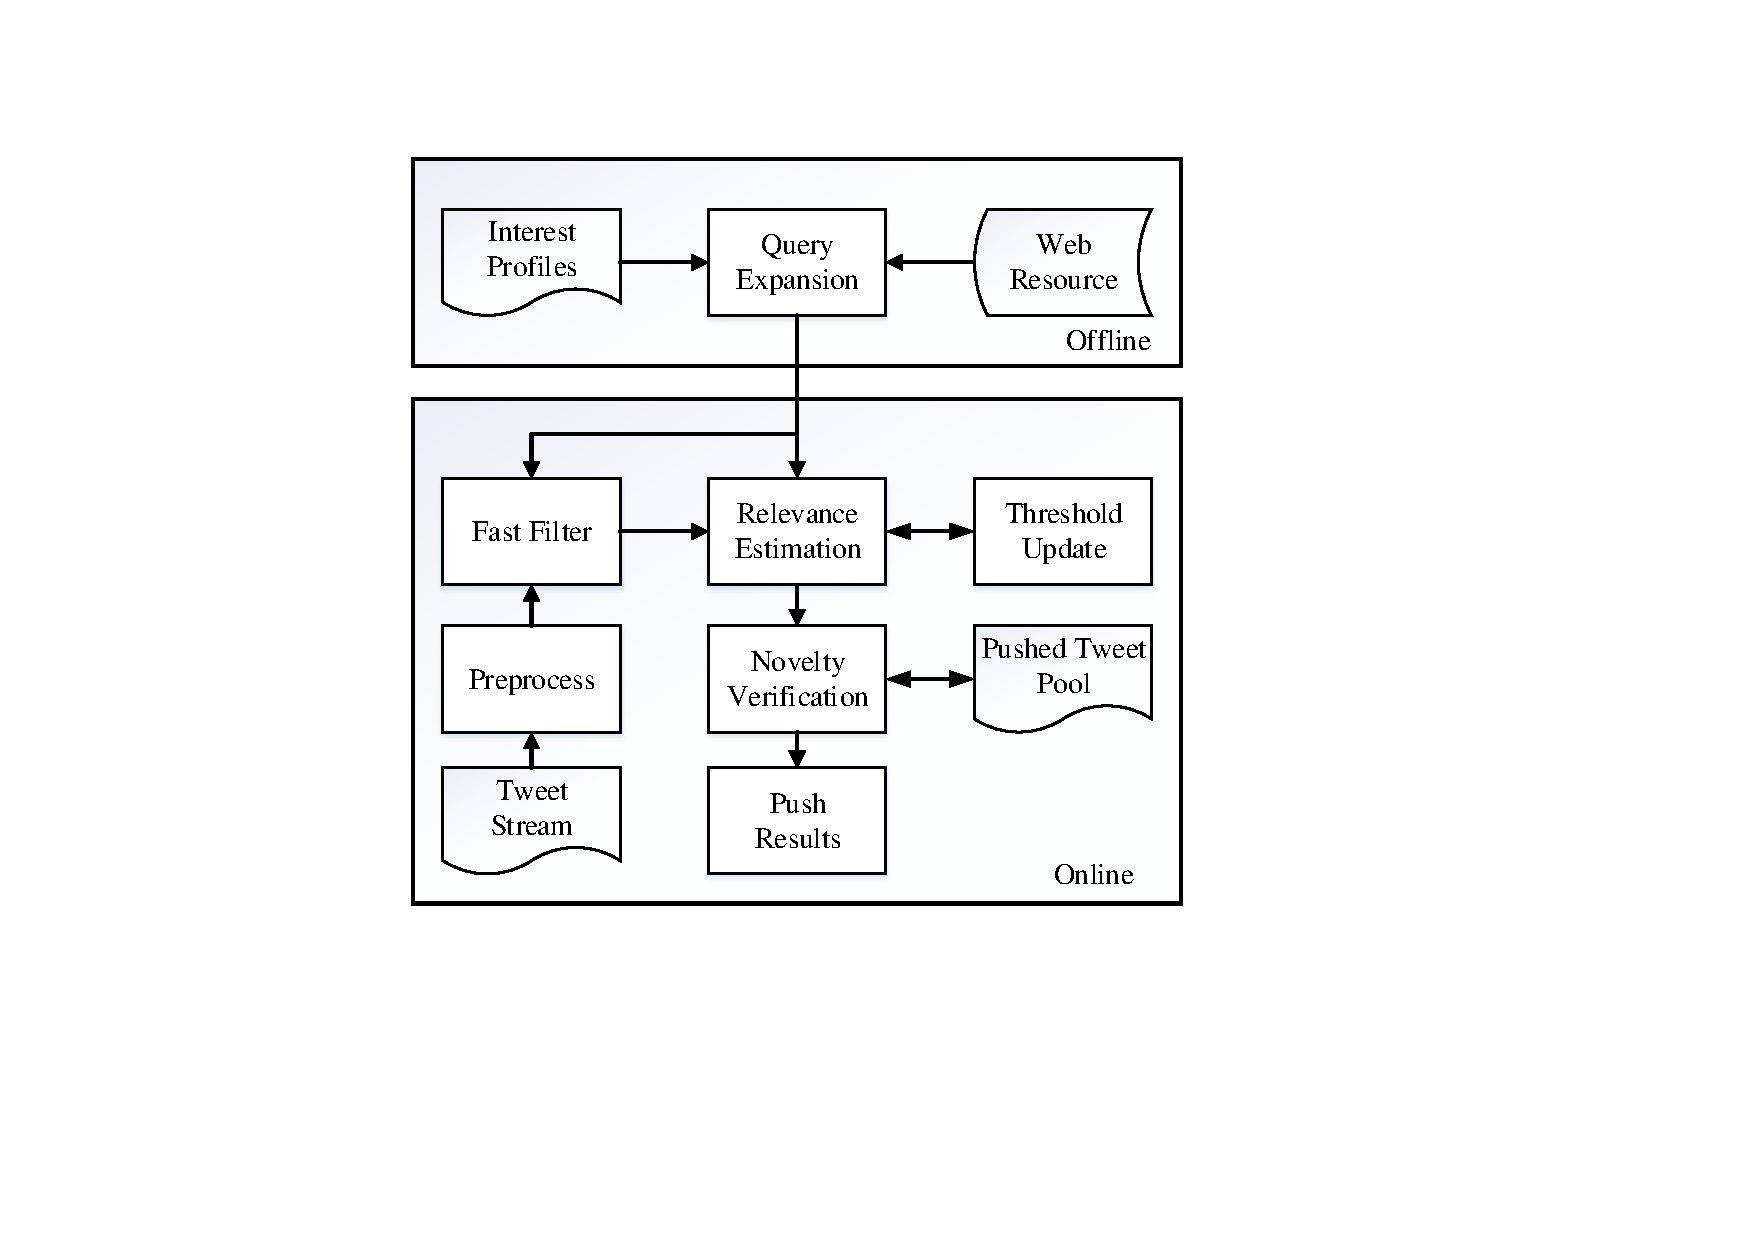
\epsfig{file=figures/scenarioA.pdf,width=0.45\textwidth}
}
\caption{Scenario A System Framework.}
\label{fig:Asys}
\end{figure}
